%%%%%%%%%%%%%%%%%%%%%%%%%%%%%%%% FIXED 
\documentclass[11pt]{article}
\usepackage{graphicx}
\usepackage[backend=biber]{biblatex}
\pagestyle{empty}
\setlength{\parskip}{0.25\baselineskip}
\renewcommand{\title}[1]{{\noindent\large\bfseries#1\medskip\\}}
\renewcommand{\author}[2]{{\noindent #1 \medskip\\ \small #2 \medskip\\}}
\usepackage[letterpaper,margin=20mm]{geometry}
%%%%%%%%%%%%%%%%%%%%%%%%%%%%%%%%

\begin{document}

\title{Exploratory Network Modelling of Complex Human Systems in Time-Use Research: Results from Wave 1 of the Singapore NCSS-NAK 360 Panel Study}
\author{
% Authors Names
Ho Han Sheng\textsuperscript{1},
Ortega Emily\textsuperscript{1},
Chan Yu Xiu Bryan\textsuperscript{1},
Tay Xunkai Azriel\textsuperscript{1},
Tang Seng Ooi Sabrina\textsuperscript{1}
}
{
% Authors Affiliations
1. School of Humanities and Behavioural Sciences, Singapore University of Social Sciences\\
}

% ABSTRACT
This study aims to examine the underlying dynamics between individual time-use patterns,  quality of life, and demographic factors (e.g., gender, income, marital status) of over 3,000 residents across 1,000 households in a 3-year longitudinal study in Singapore.

Traditional analytic strategies for time-use surveys relied on comparisons between group means, descriptive statistics, and multiple linear regression [1]. Such aggregate measures unnecessarily reduce complex human behaviour to marginal differences between subgroups - an approach antithetical to the biopsychosocial framework commonly espoused in introductory psychology modules. Accordingly, this study sought to utilise the array of network analytic methods recently refined for the modelling of complex psychological phenomena - network psychometrics, to unveil the structures undergirding human ecology. 

First, we posit that centrality and predictability measures in the context of time-use diaries represent Singaporeans' priorities in routinising their day-to-day; these were (1) work, (2) socialising, relaxation, and leisure, (3) caring for household members, and (4) household activities respectively. As data collection for this wave concluded in 2022 when COVID-19 safe distancing measures were easing in Singapore, data may reflect period-specific priorities as more returned to offices for work. We hope to compare node centralities with future waves capturing the transition to a post-COVID-19 world. 

Next, we found the presence of a strong positive conditional association between RMSSD and SDNN heart-rate variability (HRV) indices for both the female and heads of household subgroups but not for the male subgroup. This supports findings that pre-processing techniques for measuring HRV indices may have masked the moderating effects of gender on the relationship between \emph{heart rate} and heart-rate variability [2]. While gender differences in HRV have been attributed to variation in brain structures, parasympathetic modulation, and vagal activity [3], it remains open to question the similarities between heads of household (80\% men) and women that may explain this discrepancy.

Finally, this study demonstrates the promise of network psychometrics as a tool for high-dimensional exploratory data analysis beyond its initial aim of conceptualising psychopathology; and specifically the (less popular) mixed graphical model [4] for integrating and synthesising multimodal data from bio-sensors, self-reports, and demographics into a single cohesive entity. However, as is the case with Pairwise Markov Random Field Models, the link between mixed networks and causal structures remains fuzzy. While equivalence-sets and inference heuristics have been established for Gaussian Graphical Models [5], it is uncertain how the inclusion of categorical variables may affect the causal discovery process.

Altogether, this study aims to (1) broaden the applications of complex systems thinking, (2) advocate for the development of models including mixed data common in social and behavioural research, and (3) call to action for more clarity on causal inference with psychometric network models for applied researchers.

\textbf{Acknowledgements} This study was funded by the National Council of Social Services, Singapore, and Ngee Ann Kongsi, Singapore, and is part of the NCSS-NAK 360 Panel Study. NCSS does not endorse any analysis, conclusions, methods, or results created wholly by the instituition in any way, and that any such analysis, conclusion, methods, or results, are strictly the Instituition's own.

\pagebreak
{\small
\noindent[1] van Tienoven, T. P., Minnen, J., \& Spruyt, B. (2023). \textit{Time reveals everything: A glimpse into the hourglass of time use research}. ASP. \\
\noindent[2] Williams, D. P., Joseph, N., Gerardo, G. M., Hill, L. K., Koenig, J., \& Thayer, J. F. (2022). Gender differences in cardiac chronotropic control: Implications for heart rate variability research. \textit{Applied Psychophysiology and Biofeedback}, \textit{47}(1), 65-75. https://doi.org/10.1007/s10484-021-09528-w \\
\noindent[3] Koenig, J., \& Thayer, J. F. (2016). Sex differences in healthy human heart rate variability: A meta-analysis. \textit{Neuroscience \& Biobehavioral Reviews}, \textit{64}, 288-310. https://doi.org/10.1016/j.neubiorev.2016.03.007 \\
\noindent[4] Haslbeck, J. M. B., \& Waldorp, L. J. (2020). \textbf{mgm}: Estimating time-varying mixed graphical models in high-dimensional data. \textit{Journal of Statistical Software}, \textit{93}(8). https://doi.org/10.18637/jss.v093.i08 \\
\noindent[5] Ryan, O., Bringmann, L. F., \& Schuurman, N. K. (2022). The challenge of generating causal hypotheses using network models. \textit{Structural Equation Modeling: A Multidisciplinary Journal}, \textit{29}(6), 953-970. \\ https://doi.org/10.1080/10705511.2022.2056039 \\
}

\begin{figure}[h]
  \centering
  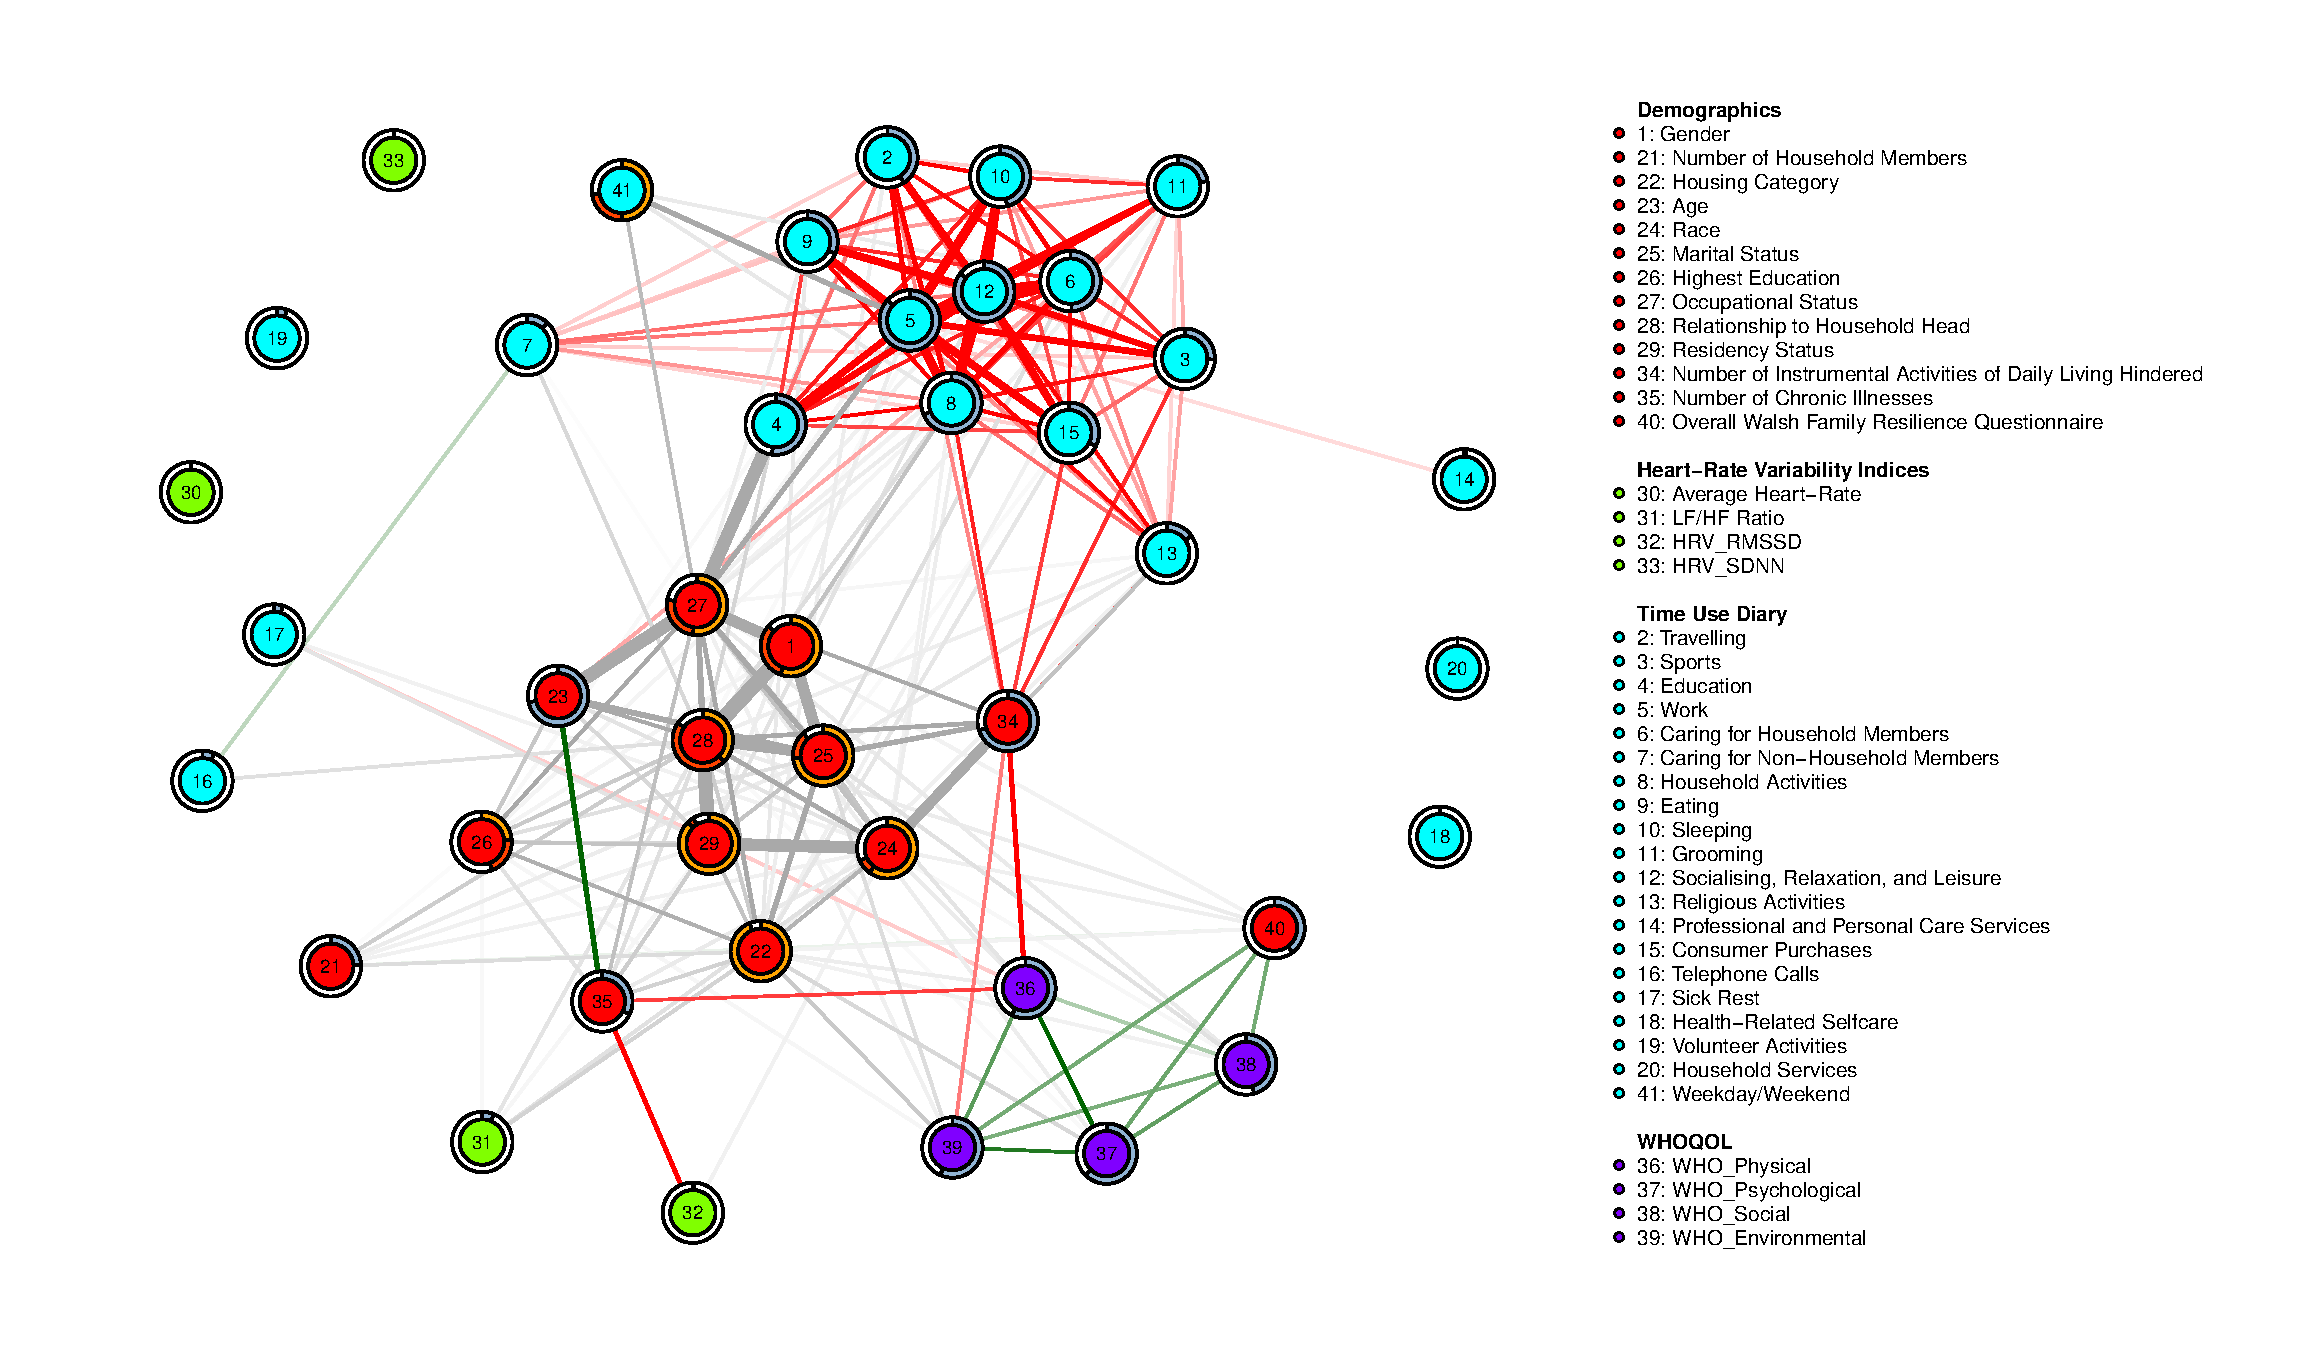
\includegraphics[width=1\textwidth]{figure.pdf}
  \caption{Mixed Graphical Model of Adults in Wave 1 (N = 2122; Weekdays = 2115; Weekends = 2096) \\
  Note: Blue rings = Proportion of variance explained; Orange rings = Accuracy, proportion of correct classification of categorical variables; Red rings = Normalised accuracy, amount of variance explained beyond accuracy
  }
\end{figure}


\end{document}